
%% bare_conf.tex
%% V1.3
%% 2007/01/11
%% by Michael Shell
%% See:
%% http://www.michaelshell.org/
%% for current contact information.
%%
%% This is a skeleton file demonstrating the use of IEEEtran.cls
%% (requires IEEEtran.cls version 1.7 or later) with an IEEE conference paper.
%%
%% Support sites:
%% http://www.michaelshell.org/tex/ieeetran/
%% http://www.ctan.org/tex-archive/macros/latex/contrib/IEEEtran/
%% and
%% http://www.ieee.org/

%%*************************************************************************
%% Legal Notice:
%% This code is offered as-is without any warranty either expressed or
%% implied; without even the implied warranty of MERCHANTABILITY or
%% FITNESS FOR A PARTICULAR PURPOSE! 
%% User assumes all risk.
%% In no event shall IEEE or any contributor to this code be liable for
%% any damages or losses, including, but not limited to, incidental,
%% consequential, or any other damages, resulting from the use or misuse
%% of any information contained here.
%%
%% All comments are the opinions of their respective authors and are not
%% necessarily endorsed by the IEEE.
%%
%% This work is distributed under the LaTeX Project Public License (LPPL)
%% ( http://www.latex-project.org/ ) version 1.3, and may be freely used,
%% distributed and modified. A copy of the LPPL, version 1.3, is included
%% in the base LaTeX documentation of all distributions of LaTeX released
%% 2003/12/01 or later.
%% Retain all contribution notices and credits.
%% ** Modified files should be clearly indicated as such, including  **
%% ** renaming them and changing author support contact information. **
%%
%% File list of work: IEEEtran.cls, IEEEtran_HOWTO.pdf, bare_adv.tex,
%%                    bare_conf.tex, bare_jrnl.tex, bare_jrnl_compsoc.tex
%%*************************************************************************

% *** Authors should verify (and, if needed, correct) their LaTeX system  ***
% *** with the testflow diagnostic prior to trusting their LaTeX platform ***
% *** with production work. IEEE's font choices can trigger bugs that do  ***
% *** not appear when using other class files.                            ***
% The testflow support page is at:
% http://www.michaelshell.org/tex/testflow/



% Note that the a4paper option is mainly intended so that authors in
% countries using A4 can easily print to A4 and see how their papers will
% look in print - the typesetting of the document will not typically be
% affected with changes in paper size (but the bottom and side margins will).
% Use the testflow package mentioned above to verify correct handling of
% both paper sizes by the user's LaTeX system.
%
% Also note that the "draftcls" or "draftclsnofoot", not "draft", option
% should be used if it is desired that the figures are to be displayed in
% draft mode.
%
\documentclass[10pt, conference, compsocconf]{IEEEtran}



\usepackage{graphicx,epsfig,subfigure}%psfrag




% Add the compsocconf option for Computer Society conferences.
%
% If IEEEtran.cls has not been installed into the LaTeX system files,
% manually specify the path to it like:
% \documentclass[conference]{../sty/IEEEtran}





% Some very useful LaTeX packages include:
% (uncomment the ones you want to load)


% *** MISC UTILITY PACKAGES ***
%
%\usepackage{ifpdf}
% Heiko Oberdiek's ifpdf.sty is very useful if you need conditional
% compilation based on whether the output is pdf or dvi.
% usage:
% \ifpdf
%   % pdf code
% \else
%   % dvi code
% \fi
% The latest version of ifpdf.sty can be obtained from:
% http://www.ctan.org/tex-archive/macros/latex/contrib/oberdiek/
% Also, note that IEEEtran.cls V1.7 and later provides a builtin
% \ifCLASSINFOpdf conditional that works the same way.
% When switching from latex to pdflatex and vice-versa, the compiler may
% have to be run twice to clear warning/error messages.






% *** CITATION PACKAGES ***
%
%\usepackage{cite}
% cite.sty was written by Donald Arseneau
% V1.6 and later of IEEEtran pre-defines the format of the cite.sty package
% \cite{} output to follow that of IEEE. Loading the cite package will
% result in citation numbers being automatically sorted and properly
% "compressed/ranged". e.g., [1], [9], [2], [7], [5], [6] without using
% cite.sty will become [1], [2], [5]--[7], [9] using cite.sty. cite.sty's
% \cite will automatically add leading space, if needed. Use cite.sty's
% noadjust option (cite.sty V3.8 and later) if you want to turn this off.
% cite.sty is already installed on most LaTeX systems. Be sure and use
% version 4.0 (2003-05-27) and later if using hyperref.sty. cite.sty does
% not currently provide for hyperlinked citations.
% The latest version can be obtained at:
% http://www.ctan.org/tex-archive/macros/latex/contrib/cite/
% The documentation is contained in the cite.sty file itself.

% *** GRAPHICS RELATED PACKAGES ***
%
\ifCLASSINFOpdf
  % \usepackage[pdftex]{graphicx}
  % declare the path(s) where your graphic files are
  % \graphicspath{{../pdf/}{../jpeg/}}
  % and their extensions so you won't have to specify these with
  % every instance of \includegraphics
  % \DeclareGraphicsExtensions{.pdf,.jpeg,.png}
\else
  % or other class option (dvipsone, dvipdf, if not using dvips). graphicx
  % will default to the driver specified in the system graphics.cfg if no
  % driver is specified.
  % \usepackage[dvips]{graphicx}
  % declare the path(s) where your graphic files are
  % \graphicspath{{../eps/}}
  % and their extensions so you won't have to specify these with
  % every instance of \includegraphics
  % \DeclareGraphicsExtensions{.eps}
\fi
% graphicx was written by David Carlisle and Sebastian Rahtz. It is
% required if you want graphics, photos, etc. graphicx.sty is already
% installed on most LaTeX systems. The latest version and documentation can
% be obtained at: 
% http://www.ctan.org/tex-archive/macros/latex/required/graphics/
% Another good source of documentation is "Using Imported Graphics in
% LaTeX2e" by Keith Reckdahl which can be found as epslatex.ps or
% epslatex.pdf at: http://www.ctan.org/tex-archive/info/
%
% latex, and pdflatex in dvi mode, support graphics in encapsulated
% postscript (.eps) format. pdflatex in pdf mode supports graphics
% in .pdf, .jpeg, .png and .mps (metapost) formats. Users should ensure
% that all non-photo figures use a vector format (.eps, .pdf, .mps) and
% not a bitmapped formats (.jpeg, .png). IEEE frowns on bitmapped formats
% which can result in "jaggedy"/blurry rendering of lines and letters as
% well as large increases in file sizes.
%
% You can find documentation about the pdfTeX application at:
% http://www.tug.org/applications/pdftex





% *** MATH PACKAGES ***
%
%\usepackage[cmex10]{amsmath}
% A popular package from the American Mathematical Society that provides
% many useful and powerful commands for dealing with mathematics. If using
% it, be sure to load this package with the cmex10 option to ensure that
% only type 1 fonts will utilized at all point sizes. Without this option,
% it is possible that some math symbols, particularly those within
% footnotes, will be rendered in bitmap form which will result in a
% document that can not be IEEE Xplore compliant!
%
% Also, note that the amsmath package sets \interdisplaylinepenalty to 10000
% thus preventing page breaks from occurring within multiline equations. Use:
%\interdisplaylinepenalty=2500
% after loading amsmath to restore such page breaks as IEEEtran.cls normally
% does. amsmath.sty is already installed on most LaTeX systems. The latest
% version and documentation can be obtained at:
% http://www.ctan.org/tex-archive/macros/latex/required/amslatex/math/





% *** SPECIALIZED LIST PACKAGES ***
%
%\usepackage{algorithmic}
% algorithmic.sty was written by Peter Williams and Rogerio Brito.
% This package provides an algorithmic environment fo describing algorithms.
% You can use the algorithmic environment in-text or within a figure
% environment to provide for a floating algorithm. Do NOT use the algorithm
% floating environment provided by algorithm.sty (by the same authors) or
% algorithm2e.sty (by Christophe Fiorio) as IEEE does not use dedicated
% algorithm float types and packages that provide these will not provide
% correct IEEE style captions. The latest version and documentation of
% algorithmic.sty can be obtained at:
% http://www.ctan.org/tex-archive/macros/latex/contrib/algorithms/
% There is also a support site at:
% http://algorithms.berlios.de/index.html
% Also of interest may be the (relatively newer and more customizable)
% algorithmicx.sty package by Szasz Janos:
% http://www.ctan.org/tex-archive/macros/latex/contrib/algorithmicx/




% *** ALIGNMENT PACKAGES ***
%
%\usepackage{array}
% Frank Mittelbach's and David Carlisle's array.sty patches and improves
% the standard LaTeX2e array and tabular environments to provide better
% appearance and additional user controls. As the default LaTeX2e table
% generation code is lacking to the point of almost being broken with
% respect to the quality of the end results, all users are strongly
% advised to use an enhanced (at the very least that provided by array.sty)
% set of table tools. array.sty is already installed on most systems. The
% latest version and documentation can be obtained at:
% http://www.ctan.org/tex-archive/macros/latex/required/tools/


%\usepackage{mdwmath}
%\usepackage{mdwtab}
% Also highly recommended is Mark Wooding's extremely powerful MDW tools,
% especially mdwmath.sty and mdwtab.sty which are used to format equations
% and tables, respectively. The MDWtools set is already installed on most
% LaTeX systems. The lastest version and documentation is available at:
% http://www.ctan.org/tex-archive/macros/latex/contrib/mdwtools/


% IEEEtran contains the IEEEeqnarray family of commands that can be used to
% generate multiline equations as well as matrices, tables, etc., of high
% quality.


%\usepackage{eqparbox}
% Also of notable interest is Scott Pakin's eqparbox package for creating
% (automatically sized) equal width boxes - aka "natural width parboxes".
% Available at:
% http://www.ctan.org/tex-archive/macros/latex/contrib/eqparbox/





% *** SUBFIGURE PACKAGES ***
%\usepackage[tight,footnotesize]{subfigure}
% subfigure.sty was written by Steven Douglas Cochran. This package makes it
% easy to put subfigures in your figures. e.g., "Figure 1a and 1b". For IEEE
% work, it is a good idea to load it with the tight package option to reduce
% the amount of white space around the subfigures. subfigure.sty is already
% installed on most LaTeX systems. The latest version and documentation can
% be obtained at:
% http://www.ctan.org/tex-archive/obsolete/macros/latex/contrib/subfigure/
% subfigure.sty has been superceeded by subfig.sty.



%\usepackage[caption=false]{caption}
%\usepackage[font=footnotesize]{subfig}
% subfig.sty, also written by Steven Douglas Cochran, is the modern
% replacement for subfigure.sty. However, subfig.sty requires and
% automatically loads Axel Sommerfeldt's caption.sty which will override
% IEEEtran.cls handling of captions and this will result in nonIEEE style
% figure/table captions. To prevent this problem, be sure and preload
% caption.sty with its "caption=false" package option. This is will preserve
% IEEEtran.cls handing of captions. Version 1.3 (2005/06/28) and later 
% (recommended due to many improvements over 1.2) of subfig.sty supports
% the caption=false option directly:
%\usepackage[caption=false,font=footnotesize]{subfig}
%
% The latest version and documentation can be obtained at:
% http://www.ctan.org/tex-archive/macros/latex/contrib/subfig/
% The latest version and documentation of caption.sty can be obtained at:
% http://www.ctan.org/tex-archive/macros/latex/contrib/caption/




% *** FLOAT PACKAGES ***
%
%\usepackage{fixltx2e}
% fixltx2e, the successor to the earlier fix2col.sty, was written by
% Frank Mittelbach and David Carlisle. This package corrects a few problems
% in the LaTeX2e kernel, the most notable of which is that in current
% LaTeX2e releases, the ordering of single and double column floats is not
% guaranteed to be preserved. Thus, an unpatched LaTeX2e can allow a
% single column figure to be placed prior to an earlier double column
% figure. The latest version and documentation can be found at:
% http://www.ctan.org/tex-archive/macros/latex/base/



%\usepackage{stfloats}
% stfloats.sty was written by Sigitas Tolusis. This package gives LaTeX2e
% the ability to do double column floats at the bottom of the page as well
% as the top. (e.g., "\begin{figure*}[!b]" is not normally possible in
% LaTeX2e). It also provides a command:
%\fnbelowfloat
% to enable the placement of footnotes below bottom floats (the standard
% LaTeX2e kernel puts them above bottom floats). This is an invasive package
% which rewrites many portions of the LaTeX2e float routines. It may not work
% with other packages that modify the LaTeX2e float routines. The latest
% version and documentation can be obtained at:
% http://www.ctan.org/tex-archive/macros/latex/contrib/sttools/
% Documentation is contained in the stfloats.sty comments as well as in the
% presfull.pdf file. Do not use the stfloats baselinefloat ability as IEEE
% does not allow \baselineskip to stretch. Authors submitting work to the
% IEEE should note that IEEE rarely uses double column equations and
% that authors should try to avoid such use. Do not be tempted to use the
% cuted.sty or midfloat.sty packages (also by Sigitas Tolusis) as IEEE does
% not format its papers in such ways.





% *** PDF, URL AND HYPERLINK PACKAGES ***
%
%\usepackage{url}
% url.sty was written by Donald Arseneau. It provides better support for
% handling and breaking URLs. url.sty is already installed on most LaTeX
% systems. The latest version can be obtained at:
% http://www.ctan.org/tex-archive/macros/latex/contrib/misc/
% Read the url.sty source comments for usage information. Basically,
% \url{my_url_here}.




% *** Do not adjust lengths that control margins, column widths, etc. ***
% *** Do not use packages that alter fonts (such as pslatex).         ***
% There should be no need to do such things with IEEEtran.cls V1.6 and later.
% (Unless specifically asked to do so by the journal or conference you plan
% to submit to, of course. )
\usepackage{fancyhdr}
\usepackage{graphicx}
\usepackage{amsmath}
\usepackage[shortlabels]{enumitem}
\pagestyle{fancy}

\rhead{Columbia University E6893 Big Data Analytics Fall 2014 Final Report}


% correct bad hyphenation here
\hyphenation{op-tical net-works semi-conduc-tor}


\begin{document}
%
% paper title
% can use linebreaks \\ within to get better formatting as desired
\title{Stock Recommendation System}


% author names and affiliations
% use a multiple column layout for up to two different
% affiliations

\author{\IEEEauthorblockN{Yuechen Qin, Bowen Dang, Zheng Fang, Guangyang Zhang}
\IEEEauthorblockA{Electrical Engineering\\
Columbia University\\
Email: zf2150@columbia.edu, gz2202@columbia.com, yq2158@columbia.edu, bd2384@columbia.edu}

}

% conference papers do not typically use \thanks and this command
% is locked out in conference mode. If really needed, such as for
% the acknowledgment of grants, issue a \IEEEoverridecommandlockouts
% after \documentclass

% for over three affiliations, or if they all won't fit within the width
% of the page, use this alternative format:
% 
%\author{\IEEEauthorblockN{Michael Shell\IEEEauthorrefmark{1},
%Homer Simpson\IEEEauthorrefmark{2},
%James Kirk\IEEEauthorrefmark{3}, 
%Montgomery Scott\IEEEauthorrefmark{3} and
%Eldon Tyrell\IEEEauthorrefmark{4}}
%\IEEEauthorblockA{\IEEEauthorrefmark{1}School of Electrical and Computer Engineering\\
%Georgia Institute of Technology,
%Atlanta, Georgia 30332--0250\\ Email: see http://www.michaelshell.org/contact.html}
%\IEEEauthorblockA{\IEEEauthorrefmark{2}Twentieth Century Fox, Springfield, USA\\
%Email: homer@thesimpsons.com}
%\IEEEauthorblockA{\IEEEauthorrefmark{3}Starfleet Academy, San Francisco, California 96678-2391\\
%Telephone: (800) 555--1212, Fax: (888) 555--1212}
%\IEEEauthorblockA{\IEEEauthorrefmark{4}Tyrell Inc., 123 Replicant Street, Los Angeles, California 90210--4321}}




% use for special paper notices
%\IEEEspecialpapernotice{(Invited Paper)}




% make the title area
\maketitle


\begin{abstract}
%Please use this template for your final report. Your final report should include following sections as this template shows. You can also include more sections if you want. The limitation of final report is 10 pages. If you would like to add additional instruction of the software package, those can be put in the Appendix and will not be counted in the 10 page limit. 

Predicting stock market movement is always difficult due to its chaotic nature. Conventionally, thumb rules and intuition seems to be the major indicator. Noticing that it might be easier to predict a stock A\rq s movement based on stock B\rq s movement,  our project proposes a general framework for multiple events to predict two stocks\rq\ dependency. By encoding a time series as a string, we can measure dependence effectively based on string distances. We apply this technique with a default criterion of maximum price follows the opening price movement for three days in succession in our project, which, can be further customised.\\

The stock recommendation system is a web application which recommends stocks with highest similarities to clients\rq\  favourites. Client view the realtime info of a specific stock and select their best-likes through drop down
buttons and search bar. The System crawls Nasdaq stock infos from Yahoo Finance in a real-time manner and
calculates similarities using Jaro Winkler Algorithm. The system recommends 5 stocks for every client favourite 
 and presents the information of these stocks in a table in UI. 
\end{abstract}

\begin{IEEEkeywords}
 components: stock; similarity; recommendation; big data; Jaro Winkler Algorithm; web application;

\end{IEEEkeywords}


% For peer review papers, you can put extra information on the cover
% page as needed:
% \ifCLASSOPTIONpeerreview
% \begin{center} \bfseries EDICS Category: 3-BBND \end{center}
% \fi
%
% For peerreview papers, this IEEEtran command inserts a page break and
% creates the second title. It will be ignored for other modes.
\IEEEpeerreviewmaketitle



\section{Introduction}

%Show motivation of your final project and a summarisation of the problem you would like to solve.
The stock market, based on real time transactions, is a new and important component of the contemporary capitalist financial system\cite{Similarity}. Recently, the number of shares trades on the stock exchange market is growing tremendously and expectations point to an even faster growth\cite{From}. Considering the scenario that the move of stock market plays an important role for companies to obtain investments, take strategic decisions and expand its activities on a global level, many specialists are motivated to take advantage of the observed behavior of shares to help avoid instability within a company, or further, to predict its behavior in the near future. Though it is possible to use the historical data of stock market to do prediction for investment\cite{Forecasting}, accurate predictions are still very hard to make due to the chaotic nature of stock markets, which might depend on external events like governmental actions, company crisis and many other factors.\\

Our project suggested a way that, instead of trying to predict one particular stock\rq s movement with respect to the whole market, it might be easier to predict a stock A\rq s movement based on stock B\rq s movement, which turned out to be the main motivation of our stock recommendation system\cite{Identifying}. Based on a customer\rq s specific choices, our system is able to recommend a number of similar stocks (both short-term results and long-term results are provided). Besides, stock trend figures and real-time stock value are all available on our system. \\

The rest of the report is structured as follows. Section II reviews the related work and presents the background to follow the report. Section III describes the system structure of our project. Section IV shows in detail how the Jaro Winkler Algorithm works in our calculation of similarity. Section V gives a overview of the software package to be open sourced. Section VI shows the experimental results obtained by our recommendation and Section VII presents the conclusions.


% no \IEEEPARstart

% You must have at least 2 lines in the paragraph with the drop letter
% (should never be an issue)

\section{Related Works}

%Mention previous works related to the problem you would like to solve.

Much research efforts has gone into the field of similarity-based approach for stock prediction. In stock market analysis, the behavior of share pricing is usually described by discrete-time series, where each term of the series is a set of attributes regarding the price variations\cite{Similarity}. The indicators, Price Ratio and Price Comparison do compare two stocks\rq\  prices, but this is for finding strong stocks rather than dependencies between stocks. People have used clustering techniques\cite{Which}, mining association rules from database of transactions\cite{Mining} and geometric properties\cite{Principles}\cite{Time} to find stock similarity. The metric distances and methods based on topological properties and random matrix theory have also been used for the purpose.\\

The representation of time series as an univariate linear stochastic process is the development basis of the Autoregressive Model (AR) and the Moving Average Model (MA), both members of the Autoregressive Integrated Moving Average (ARIMA) model\cite{Econometric}, which has been one of the most popular approaches to time series forecasting. The ARIMA model takes advantage of both weak-stationary and non-stationary properties of time series and proposes to integrate autoregressive and moving averages, offering ways to identify seasonalities observed at the series micro-level. It is based on three parameters: lags of difference, the difference order term and the lags of forecast errors.\\

When non-linearities are present in the data, non-linear methods including the Autoregressive Conditional Heteroskedasticity (ARCH) method and its variations are adopted to model share price behavior\cite{Arch}. These models have some drawbacks, such as the lack of scalability of the HMM technique and the limitation of the method of Analogues to handle long periods of time and high-dimensionality series.\\

Soft-computing approaches based on artificial intelligence methods have suggested new ways to forecast time series outcomes\cite{Fast}. These methods usually aim to predict trends using a classifier that gives an interpretation of summarized data. Among these approaches, Artificial Neural Networks (ANN) have been one of the most popular tools used in recent works regarding the financial market.



\section{System Overview}
%Describe your system design. Datasets can be described here.
\begin{enumerate}[label=\Alph*]

%skeleton
\item \textit{System Structure}

 We designed a stock recommendation system which can recommend stocks with highest similarities to clients? favourites. The system uses a J2EE     framework, it has one UI page,  several serve lets, a recommendation algorithm called "Jaro Winkler" algorithm  and a mysql database. Figure 1 shows an overview of project structure. The project components are explained in detail in the following:\\
           
           UI and servlets:\\
           The UI helps clients choose their favourite stocks through drop-down buttons and search bar. They can view the realtime trend of every stock by clicking the \textbf{plot} button. The drop down buttons helps them make a multiple selections based on that suits their requirement. After client makes their own choices, the UI will send client favourites to the back-end and present recommendation results from back-end in a table. Our  UI is written in html and is decorated with  CSS and Bootstrap. It has a group of javascript functions to interact with clients in a dynamic manner.\\
Servlets connect UI and java code block of the project. It passes the input from UI to a java program and hands out the return data from java program to the UI. The project contains four servlets, which is used to calcite similarity, calculate distance between two stocks and extract stock information from Yahoo Finance.\\ 

          Yahoo Finance API:\\
           We crawls Nasdaq stock information from the Yahoo Finance API. The URL of this API is "http://finance.yahoo.com/d/quotes.csv?s=". We select bid, 50 day moving average, day high and day low as our attributes and store these informations into our database.\\
                         
            java blocks:\\
              The system has two java packages, which are: data model and similarity calculation model. \\
              The data model are the classes we used to store and process the stock information locally. For each clients' best-like stock, the system builds up a CustomerStock object to store its symbol and a list which contains 5 recommended stocks with the highest similarities to it. Every recommended stock is stored in the recommendation list as a RecStock object. It contains fields such as its similarity to clients' favourites, its bid, moving average, day high and day low. \\
              
              The similarity calculation model are the java programs we used to calculate similarity. 

          
 \begin{figure}[!h]
            \centering
           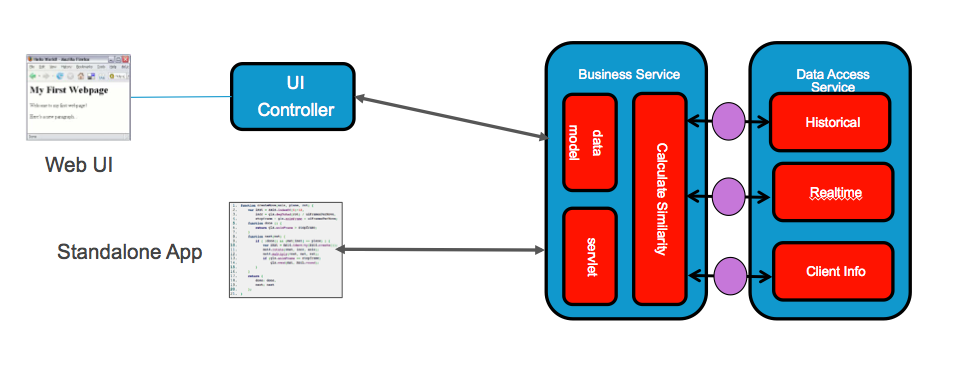
\includegraphics[width=0.5\textwidth]{figures/skeleton.jpg}
           \caption{System Structure}
          \vspace{0.1cm}
    \end{figure}
    
     \begin{figure}[!h]
            \centering
           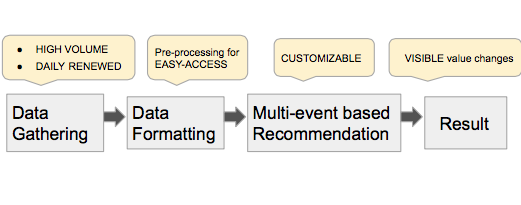
\includegraphics[width=0.5\textwidth]{figures/flow.jpg}
           \caption{Flow map}
          \vspace{0.1cm}
    \end{figure}
 
    
    
   %dataset 
   \item  \textit{Dataset}\\

We use NASDAQ Stock Exchange Data as our dataset. It contains 2959 stocks in total. As mentioned above, we use Yahoo Finance dataset to acquire historical prices of each stock. The dataset is daily renewed  with most recent value via Yahoo API.\\
           We choose MYSQL as our database because it is the most popular open source database and it is most deployed database in the web and cloud( with 80\% deployments integrated)
   \begin{figure}[!h]
            \centering
           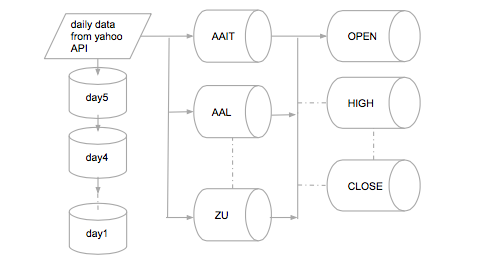
\includegraphics[width=0.5\textwidth]{figures/dataset.jpg}
           \caption{Dataset}
          \vspace{0.1cm}
    \end{figure}

    
 \end{enumerate}

\section{Algorithm (you can change this section name)} 

%Describe the software package that is going to be open sourced. Show some screen shots of how user use it and or UI.
Manilla et. al. introduced the idea of an event for time series in [2]. An event is an occurrence of a particular type which has a time stamp attached to it. Given a set $\overline{E}$ of event types, an event $\alpha$ is a pair of $\left ( e,t \right )\in \overline{E}$, where e is an event tye and t is an integer. the occurrence time of the event.Mathematically, a time series can be seen as an ordered sequence of events $\left \{ \alpha_{i}  \right \}=\left \{ e_{i},t_{i} \right \}$ where $e_{i}$ is an occurrence of a particular type and $t_{i}$ is the time stamp.For stock time series, the set of event types can be (daily opening price, daily closing price, daily trading volume, daily high price and daily low price) and the time series can be described as any of these four event types by giving the value associated with the date. \\
\par 
An episode is a sequence of events.Manilla et. al. defines an episode as a triple $\left (V,< ,g  \right )$ where $V$ is a set of nodes and $<$ is a partial order of $V$, and $g:V\rightarrow \overline{E}$ is a mapping associating each node with an event type.\\
Note that stock history can be seen as a series of events, we are able to define an episode as a predefined sequence of events. For example, considering "daily volume" as an specific event,we can define an episode "three successive days of volume increase"($T_{i}<T_{i+1}<T_{i+2}$, $T_{i}=$ Trading Volume value on $i^{th}$ day). If we can define stock move in a time wondow as a single episode, we are able to analyze its property more easily.
\par
However, we notice that an episode is only defined by a specific event type and its ordering.However, it is far from enough for a complex market. For example, we are not able to define "high price follows the move of open price"($(O_{i+1}-O_{i})*(H_{i+1}-H_{i})>0$, $O_{i})=$ Trading open value on $i^{th}$ day and $H_{i})=$ Trading high value on $i^{th}$ day) as an episode using the above definition.This problem is because that an episode depends on a single event. To solve this problem, we now extend the space of a single event to a multi-event set.We now define our new event set as follows:
\par
$E=\left \{ (e_{1},t_{1}),...,(e_{i},t_{i}),(e_{l},t_{l}) \right \}$, $\forall i=(1,2,...,l)$
\par
$e_{i}=\left \{ s_{1},...s_{k},q:s_{m}\leftrightarrow s_{n} \right \}$, $\forall m,n=(1,2,...,k)$
\par
where $q$ is a set of mapping among events in event set $e_{i}$, which implies a complex relationship amoung stock events such like open price and volume.
\par
Give this definition of a complex event, we are now able to find multi-event episodes from stock time series, as show in the following:
\vspace{1.2mm}
\par
1. Read time series $S\left ( t \right )$, $t=1,...,N$
\par
2. Read episode definition 
\par\quad $E=\left \{ (e_{1},t_{1}),...,(e_{i},t_{i}),(e_{l},t_{l}) \right \}$, $\forall i=(1,2,...,l)$
\par
3. episode\_index = 1
\par\quad complementary\_episode\_index = 1
\par
4. for every event $e_{i}$ do
\par\quad if $e_{i}$ is an valid event at time $t_{i}$
\par\quad push $(e_{i},t_{i})$ to valid\_times$\left [ j \right ]$
\par\quad end if  end for
\par
5. find combinations of $(e_{i},t_{i}), i=1,...,m$ that either $q$ 
\par\quad or complements of $q$ is satisfied
\par\quad If $q$ is satisfied, push that to 
\par\quad episode$[$episode\_index$]$ episode\_index++;
\par\quad end if
\par\quad If complements of $q$ is satisfied, push that to 
\par\quad complementary\_episode$[$complementary\_episode\_index$]$
\par\quad complementary\_episode\_index++;
\par\quad end if
\vspace{1.2mm}
\par
After we have defined the multi-event episode, we are able to define a specific event set with a single symbol. For example, if we would like to check the inner relationship between two stocks that "high price and low price has a negative relationship
within a week's period", we are able to define this episode as event "a" and its counterexample as event "b". The algorithm we use for encoding is as follows,
\par
\vspace{0.6mm}
1. Read episode 
\par\quad $E=\left \{ (e_{1},t_{1}),..,(e_{l},t_{l}) \right \}$, $\forall i=(1,2,...,l)$
2. $B=\emptyset$
\par\quad for each $i=1,...N$, $N=$ lehgth of checked time series, 
\par\quad do
\par\quad if $t_{i}$ belongs to a member of episode description
\par\quad $B=B.append("a")$
\par\quad else if $t_{i}$ belongs to a member of complementary 
\par\quad episode description
\par\quad $B=B.append("b")$
\par\quad else
\par\quad $B=B.append("c")$
\par\quad end do
\par
3. return $B$
\vspace{0.6mm}
\par
This way, we can turn time series comparison problems into a string similarity checking.After we've got two equivalent ternary strings, similarity between these two stocks can simply seen as measured string distance, which will be discussed later. \\
\par
In our further study, we find that these multi-event question can be altered to a combination of a set of single events, so we look back to our initial definition of event set and notice their inner relationship. Now that we are using static event to do similarity evaluation, we are able to alter a complex language to a much simpler combination of equalization checking. For example, we can abstract most of the restrictions as combinations of "in a $k$ day window, $s_{m}$ and $s_{n}$ has a negative/positive relation", which means that it will be more efficient for us to deal with the large amount of stock data if we have a pre-encoded event description. That way, we only have to add the mapping information every time we want to check a different property or inner relationship of the stock market. Our pre-encoded content of each event set like in the following:\\
\vspace{1.2mm}
\par
1. Read episode 
\par\quad $E=\left \{ (e_{1},t_{1}),..,(e_{l},t_{l}) \right \}$, $\forall i=(1,2,...,l)$ and
\par\quad $e_{i}=\left \{ s_{1},...s_{k},q:s_{m}\leftrightarrow s_{n} \right \}$, $\forall m,n=(1,2,...,k)$
\par
2. $A_{1},...A_{k}=\emptyset$
\par\quad for each $j=1,...k$, $k=$ length of event space, do
\par\quad for each $i=1,...N$, $N=$ length of checked time series,
\par\quad do
\par\quad if $s_{j}$ belongs to a member of episode description
\par\quad $A_{j}=A_{j}.append("a")$
\par\quad else if $t_{i}$ belongs to a member of complementary
\par\quad episode description
\par\quad $A_{j}=A_{j}.append("b")$
\par\quad else $A_{j}=A_{j}.append("c")$
\par\quad end do 
\par\quad return $A_{j}$ 
\par\quad end do
\par
3.Alter $q:s_{m}\leftrightarrow s_{n} $ to $Q:A_{m}\leftrightarrow A_{n}$
\par 
4. return $E_{i}=\left \{ A_{1},...A_{k},Q:A_{m}\leftrightarrow A_{n} \right \}$
\vspace{1.2mm}
\par
In the above encoding, we use Jaro-Winkle algorithm to check whether $s_{j}$ is a member of episode description or its complement. It is also used for our future comparison work. Jaro(see e.g., Winkler 1985, 1989, Winkle and Thibaudeau 1990) introduced this string comparator to measure the aprtial agreement between two strings. The string comparison algorithm accounts for length of strings and partially accounts for the types of errors typically made in alphanumeric strings by human beings. It is used to adjust exact agreement weights when two strings do not agree on a character-by-character basis.
\par
Specifically, the Jaro string comparator is
\vspace{2mm}
\par\quad  $d_{j}=\left\{\begin{matrix}
0 & if\: \: \: m=0\\ 
\frac{1}{3}(\frac{m}{\left | s_{1} \right |}+\frac{m}{\left | s_{2} \right |}+\frac{m-t}{\left | s_{1} \right |}) & otherwise
\end{matrix}\right. $
\par where 
\par\quad $m$ is the number of matching characters
\par\quad $t$ is the number of transpositions
\par\quad $\left | s_{1} \right |$ is the length of string in first file 
\par\quad $\left | s_{2} \right |$ is the length of string in second file
\vspace{1.2mm}
\par Two characters are considered in common only if they are no further apart than $L/2-1$ where $L = \max(\left | s_{1} \right |,\left |s_{2}  \right |)$.
\par
Jaro–Winkler distance uses a prefix scale $p$ which gives more favourable ratings to strings that match from the beginning for a set prefix length $\ell$. Given two strings $s_{1}$ and $s_{2}$, their Jaro–Winkler distance $d_{w}$ is:
\par\quad $d_{w}=d_{j}+(\ell p(1-d_{j}))$
\par where
\par\quad $\ell$ is the length of common prefix at the start of the string up to a maximum of 4 characters
\par\quad $p$ is a constant scaling factor for how much the score is adjusted upwards for having common prefixes
\par 
In our preparation work, we encode the episode we want to check as a string, of which the length is the time window. we have realized Jaro\_Winkle algorothm, we are able to check whether $s_{j}$ is a member of episode description or its complement by doing the following:
\vspace{1.2mm}
\par\quad if $s_{j}=string\_episode$
\par\quad $A_{j}=A_{j}.append("a")$
\par\quad else if 
\par\quad $Jaro\_Winkle.compare(t_{i},string\_episode)=0$
\par\quad $A_{j}=A_{j}.append("b")$
\par\quad else $A_{j}=A_{j}.append("c")$
\par\quad end if
\vspace{1.2mm}
\par
After we look deeper into our encoding process and analyze the experimental result,we notice that the condition $e_{i}$ belongs to neither a member of episode description nor its complement will bring a considerable impact on checking the similarity when we increase the window length such like episode "In a 2 week period, trading volume will follow the move of open price". Also considering the property of JarO\_Winkle algorithm, we do the following change to our encoding algorithm:
\vspace{1.2mm}
\par
1. Read episode 
\par\quad $E=\left \{ (e_{1},t_{1}),..,(e_{l},t_{l}) \right \}$, $\forall i=(1,2,...,l)$
2. $B=\emptyset$
\par\quad for each $i=1,...N$, $N=$ lehgth of checked time series, 
\par\quad do
\par\quad if $t_{i}$ belongs to a member of episode description
\par\quad $B=B.append("a")$
\par\quad else if $t_{i}$ belongs to a member of complementary 
\par\quad episode description
\par\quad $B=B.append("b")$
\par\quad else if $episode\_window<4$ ,where
\par\quad $episode\_window$ is the number of days included in an 
\par\quad episode
\par\quad $B=B.append("c")$
\par\quad end do
\par
3. return $B$
\vspace{0.6mm}
\par


\section{Software Package Description}
%UI overview

\begin{enumerate}[label=\Alph*]
 
 %UI overview
  \item  \textit{UI overview}

The User interface of our stock recommendation system contains our project title, main page figure, three drop-down buttons and recommendation search bar.  The function of these components are explained in detail in the following.\\
           \begin{figure}[!h]
            \centering
           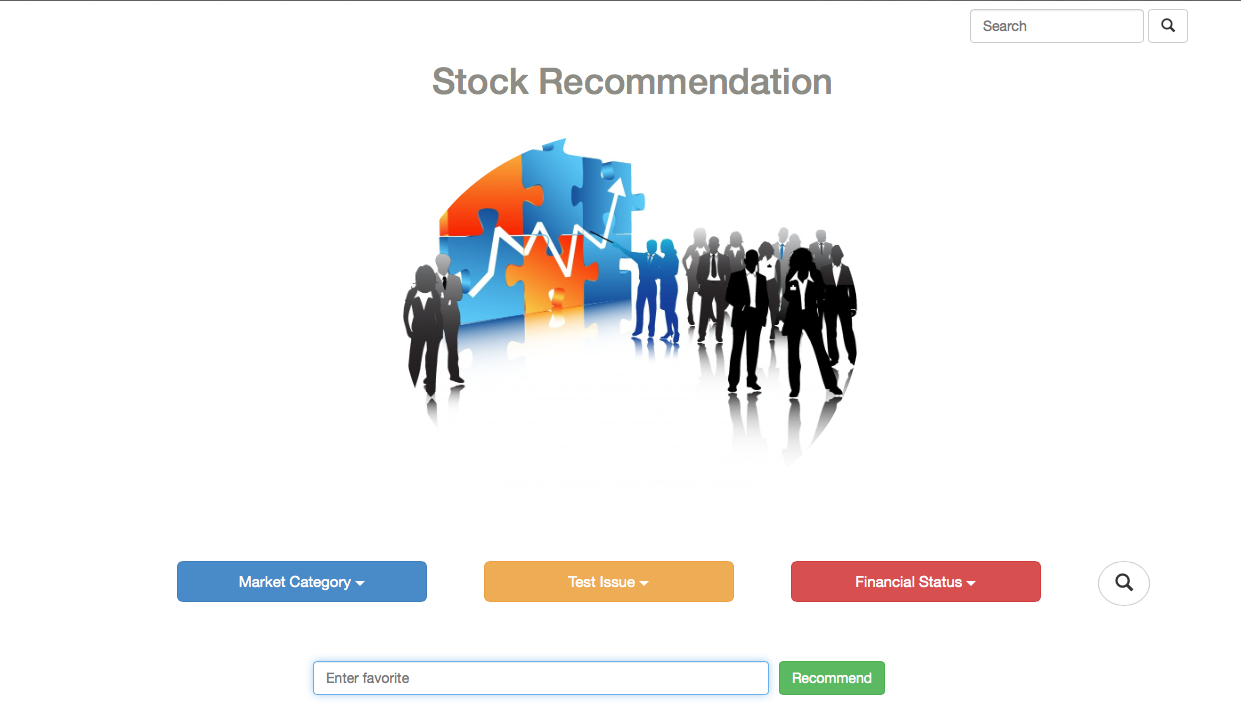
\includegraphics[width=0.5\textwidth]{figures/UI_overview.jpg}
           \caption{UI overview}
          \vspace{0.1cm}
    \end{figure}

    
    
%drop down button    
 \item  \textit{Drop down button}

 The first step of our recommendation process is to let the client choose his favourite stocks. Clients can make selections through the three drop-down buttons, which are market category, test issue and finical status. When client chooses different options, the content of the related search bar will also change.  On the right side of the drop-down buttons there is a round search button, a table is extracted from our database which presents all the stocks that fit in the prerequisites. \\
 \begin{figure}[!h]
            \centering
           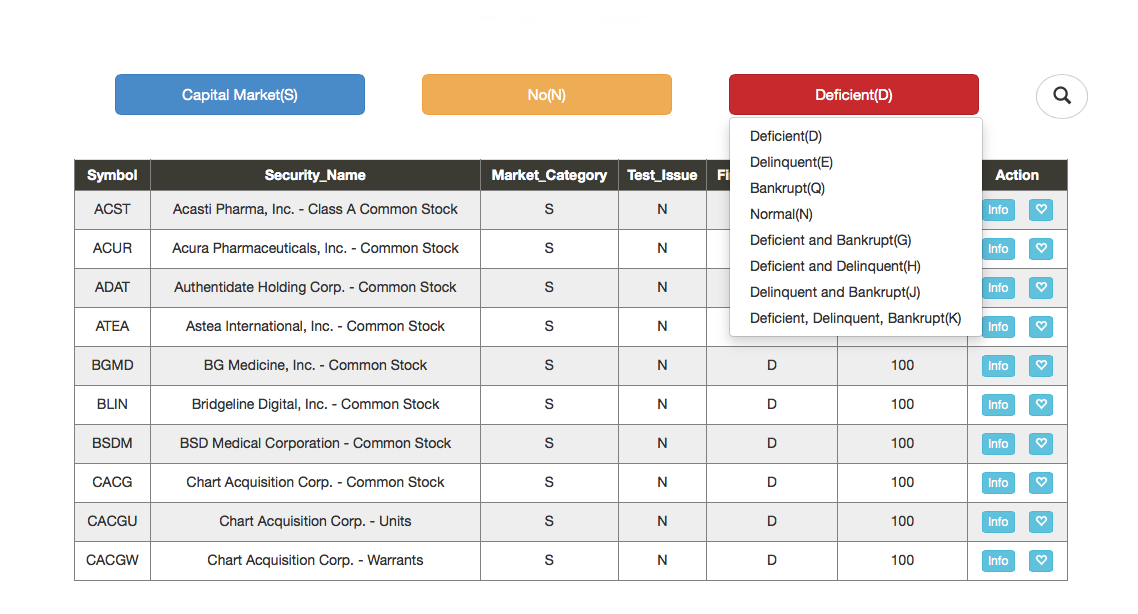
\includegraphics[width=0.5\textwidth]{figures/drop_down_button.jpg}
           \caption{Drop down buttons}
          \vspace{0.1cm}
    \end{figure}

   
   

 
    
%recommendation
 \item  \textit{Recommendation}
 
          Suppose that the client has chosen two stocks as his favourites, after he clicking the \textbf{recommend} button, the system send the information to the back-end, which will calculate the similarities of all the stocks from Nasdaq stock market to the two stocks and presents the results in a table.\\
           
 The system recommends 5 stocks with highest similarities for every choice. The table also presents the general information for the recommended stocks such as similarity, todays bid, moving average, day high and day low.\\

  \begin{figure}[!h]
            \centering
           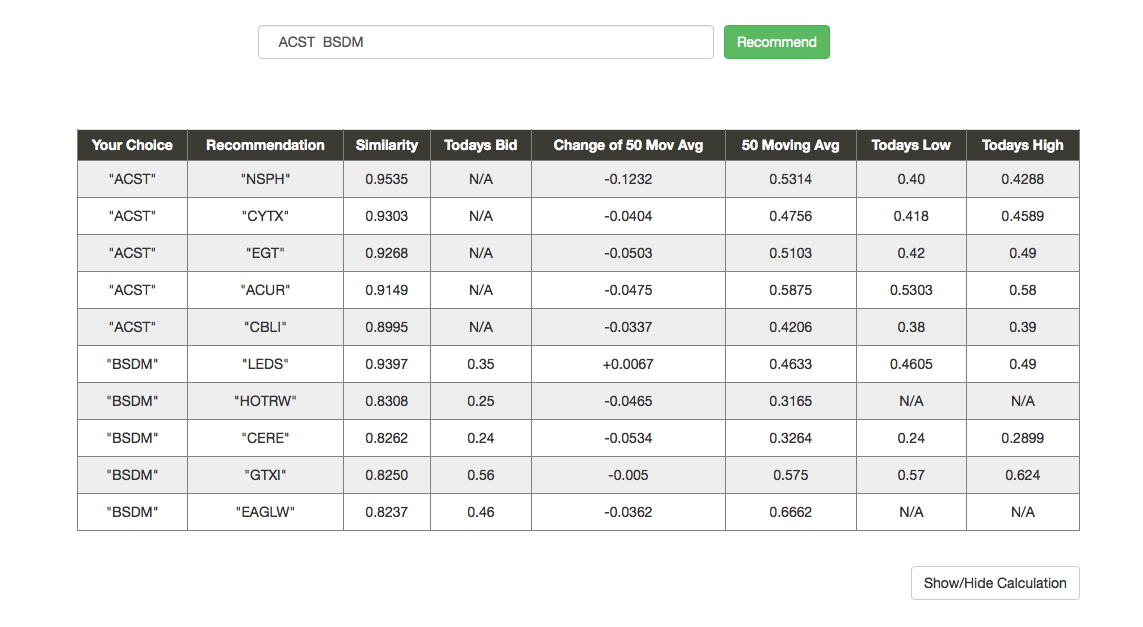
\includegraphics[width=0.5\textwidth]{figures/recommendation.jpg}
           \caption{Recommendation results}
          \vspace{0.1cm}
    \end{figure}

    
   %search button 
   \item  \textit{Search Button}

 Additionally, we also have a search bar, which is used to search for a specific stock.  If you type \textbf{AAPL} in the search bar, it will show you the stock information of apple. The format is exactly the same as the result of \textbf{info} button.\\
   \begin{figure}[!h]
            \centering
           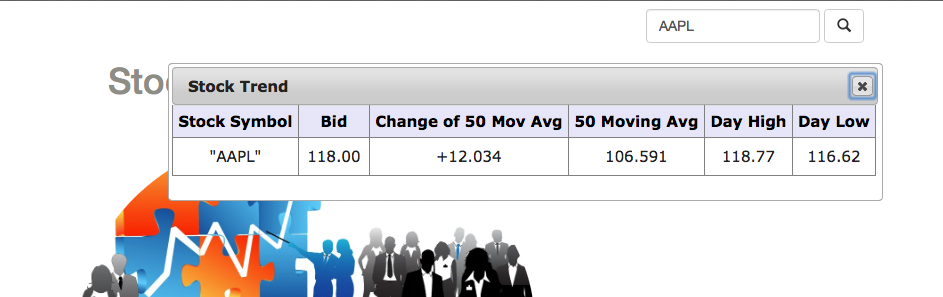
\includegraphics[width=0.5\textwidth]{figures/search_button.jpg}
           \caption{Search results}
          \vspace{0.1cm}
    \end{figure}

    
    %plot button
      \item  \textit{Info and like button}
      
   In the last cell of each row, we have two function buttons: \textbf{info} and $\heartsuit$. 
   The $\heartsuit$ is clicked if the client likes the stock. When client clicks the $\heartsuit$  button, the symbol of the stock will be automatically added to the recommendation search bar.\\
    Finally, if you want to see the historical line graph of a stock, just click on the \textbf{info} button and then the line graph is presented as in Figure 1.

% info button
 \begin{figure}[!h]
            \centering
           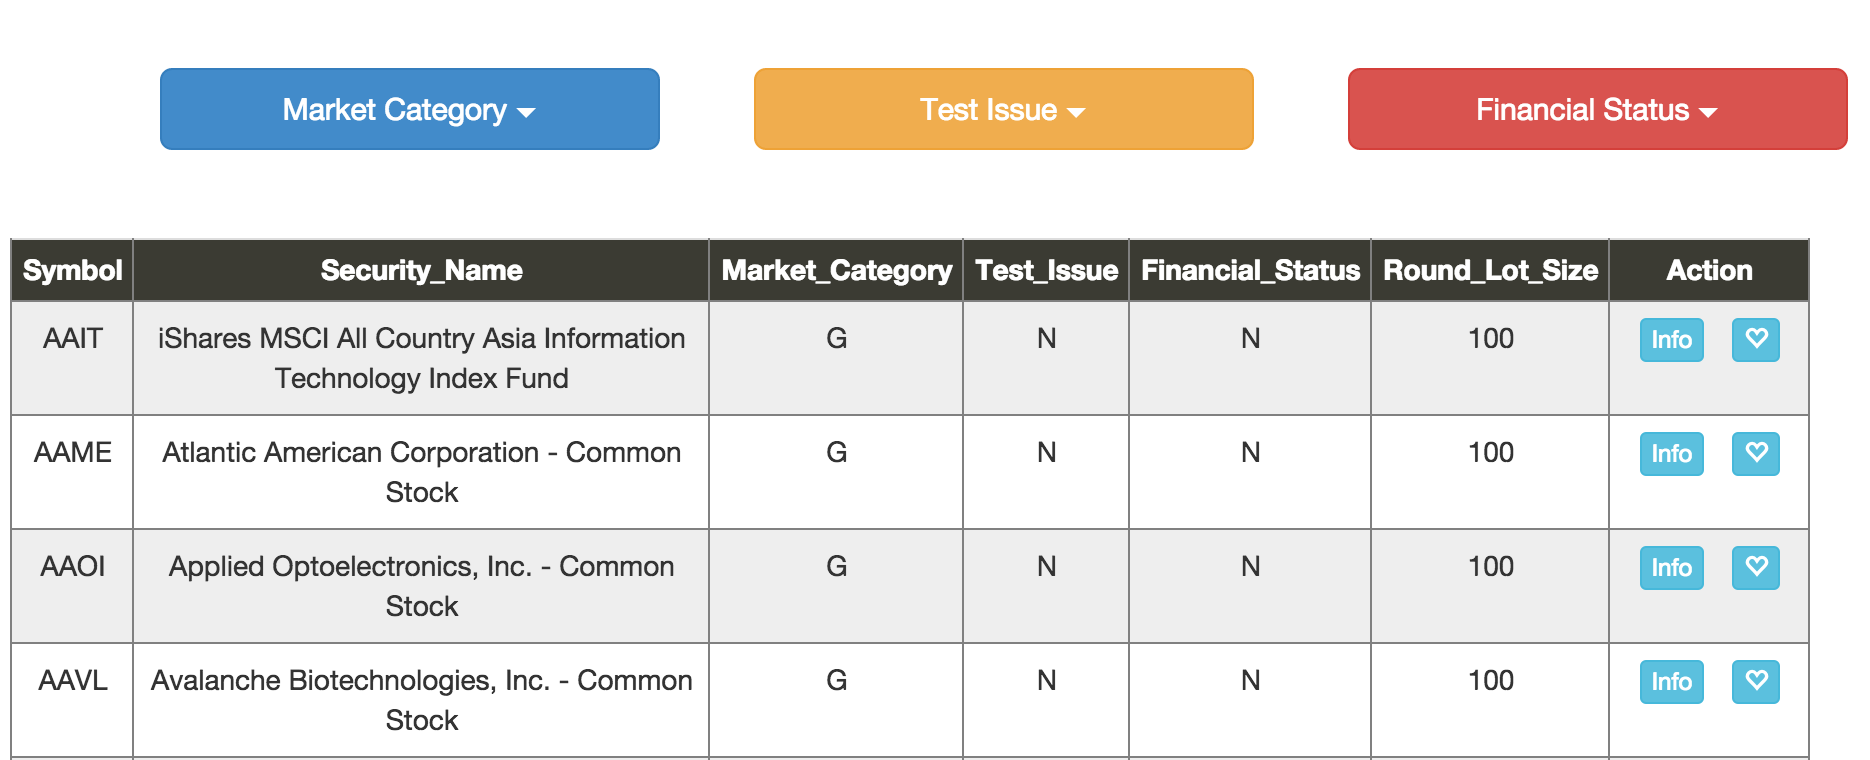
\includegraphics[width=0.5\textwidth]{figures/info_button.png}
           \caption{info button}
          \vspace{0.1cm}
 \end{figure}
 
 % historical line chart
 \begin{figure}[!h]
            \centering
           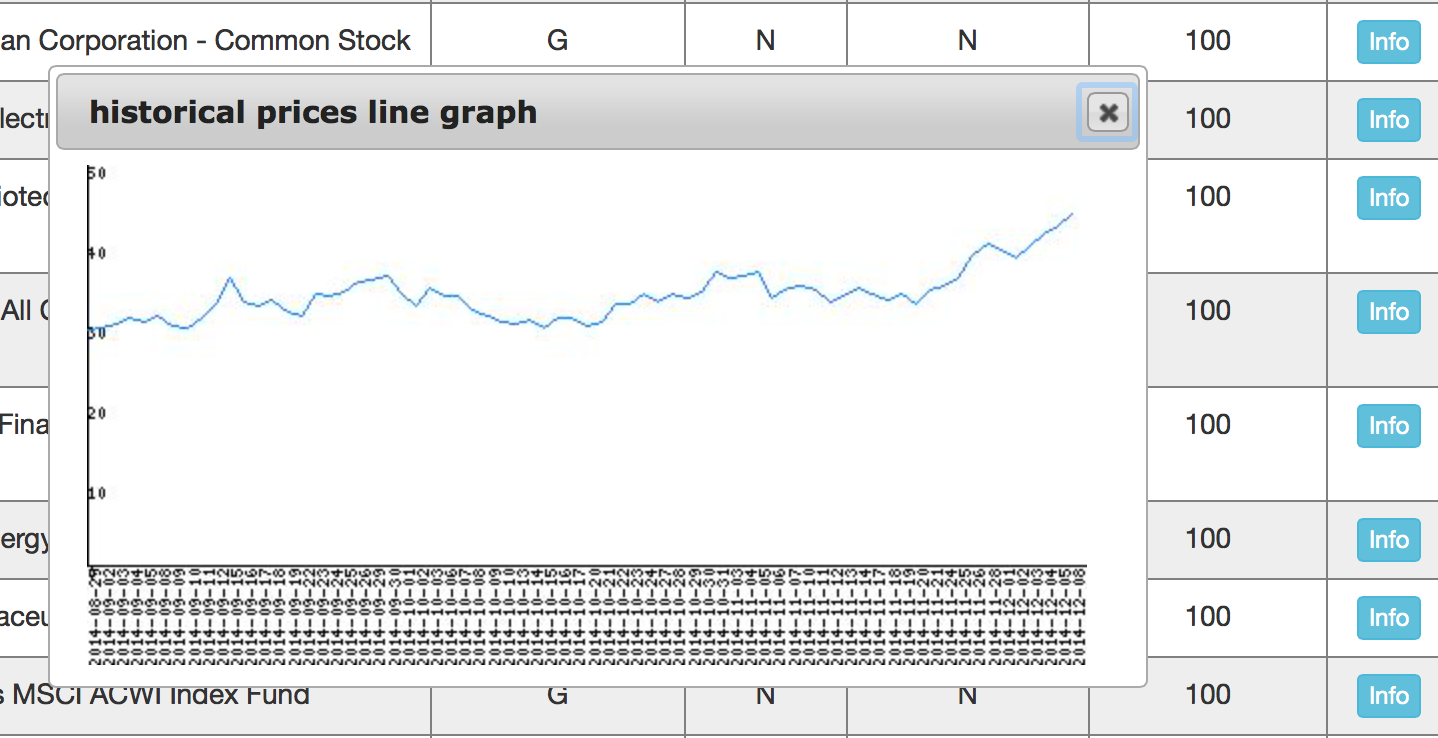
\includegraphics[width=0.5\textwidth]{figures/line_chart.png}
           \caption{line chart}
          \vspace{0.1cm}
 \end{figure}

As is shown in Figure 2, a dialog called "historical prices line graph" pops up when clicking the "info" button. The horizontal coordinate stands for the dates and the vertical coordinate stands for the open prices of the selected dates. The number of recent days' price, which shows the trend of the stock price, can be helpful for stock buyers to get a general sense of the chosen stock.\\


We decide to realize our purpose using the following steps: \\
\indent1) to connect to the  MySQL database and draw a line chart and store it using PHP; \\
\indent2) to use the HTML file to invoke the PHP file and pass to it the parameters; \\
\indent3) to fetch and show the line chart drawn via a HTML file. \\
\indent We use PHP to connect to the MySQL database and draw the line chart using the historical stock prices. And then use html to call and execute the PHP file so that the picture can be presented.


The reason why I choose PHP to draw the picture is that it is easy to connect to the database and to draw a picture at the front end. First, I use the mysql\_connect() function to connect to the database. Then I use mysql\_select\_db() function to choose the stock database. I use the following statements to receive the symbol transmitted from HTML to get the symbol of the stock for the query: 


\$symbol = \$\_GET['symbol'];

\$sym = (string)\$symbol."\_NASDAQ";

Then I utilize mysql\_query() function to fetch the date and open price of the given stock by its symbol. After getting the data, I use the mysql\_fetch\_row() function to traverse the rows of the given table and then array\_slice() to get the latest given number of days' stock price data.\\


Having fetched the data needed, we begin to draw the line chart. In the first place, I use the associative array \$price to store the data with key equal to date and value equal to the stock price. 
To initialize, use the imagecreatetruecolor() to create a new true color image, imagecolorallocate() to set the colors, and imagefill() to perform a flood fill starting at the given coordinate with the given color in the image. I set the total image to be 500 by 300 pixels. X-axis and Y-axis labels can be easily set by imagestringup() function with iterations. And then I can draw the X axis and Y axis using imageline() function. The following key step is to convert the \$price associative array to the \$point associative array in order to make the stock price correspond to the pixels of the image so that I can draw the picture. Lastly, I use imagesetpixel() to draw the dots and imageline() to connect the dots with lines. The jpeg image can be created using imagejpeg() function and stored to the designated directory. \\


The last thing is to make sure the PHP file is connected and can be invoked by the HTML file which creates our GUI. We use JavaScript to program the behavior of web pages. I create a function called  plot() to be called when the button "info" is clicked. The symbol of the stock is stored in the "value" variable as described by the following 2 statements:\\


var cell=document.getElementById("t02").rows[a].cells;

var value=cell[0].innerHTML;

We use xmlhttp.open("GET","http://localhost/plot\_400\_30\\0.php?symbol="+value,true) function to call the "plot\_400\_300.php" file and to pass the "symbol" parameter to the PHP file. To solve the time delay between the drawing and storing functions and the fetching and displaying functions, we decide to store our line chart under the web content of eclipse working directory in order to use eclipse's automatic refreshing feature. \\
   
   
\end{enumerate}

    
          

\section{Experiment Results}
%Describe the experiment results of your algorithm. Show how did you evaluate the performance of your algorithm.
We are now able to use rather complex episodes for our stock market evaluation. Since it is hard for us to get access to commercial databases, we use stock information  provided by yahoo finance to show that our similarity evaluation is reasonable.\\

\par 
As discussed before, our system is able to recommend 5 most similar stocks for investors based on user defined episode criterion. In our following experiment, we set our basic episode "high price will have a positive relationship with open price in a $k$ day period", and we set different $k$ value and training data space to see the performance of our recommendation. With this criterion, similarity between stock A and stock B implies that their three day following patterns are similar. So if short trading on A is profitable, we can expect a profitable trading on B soon after.\\
\par 
In our experiment, we randomly pick stock JSM for further evaluation.Because of space constraint, we give a representation of the most similar 3 stocks. We first choose 50 days data as our training data and set the time window $k=$ 3.The open and high price of JSM in the last 50 days is shown in Figure 11. \\
\par
\vspace{2mm}
 \begin{figure}[!h]
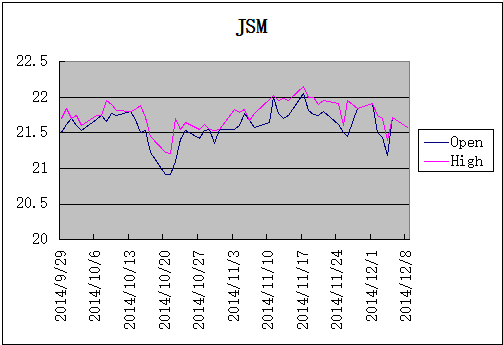
\includegraphics[width=3in]{figures/JSM}
\caption{Stock time series snapshot for JSM}
\vspace{2mm}
 \end{figure}
\par

\vspace{1mm}
\par
Our recommendation result are stock IEP, CTRP and BDSI, as shown in Figure 2, Figure 3 and Figure 4. As we can clearly see from the figures, stock IEP and JSM shows high cirrelation, their trend line suggests a good similarity. Also, if we look at some specific area in the figures around 2014/10/20, 2014/11/17 and 2014/12/8, we will find that the trend of our recommended stocks all have similar trend as our selected stock, which means that our recommendation is helpful in deciding similar stocks.\\
\par
\vspace{2mm}
 \begin{figure}[!h]
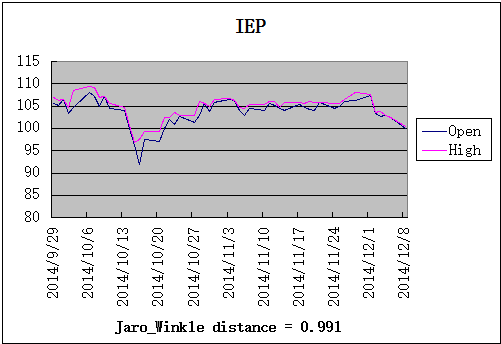
\includegraphics[width=3in]{figures/IEP}
\caption{Stock time series snapshot for IEP}
\vspace{1mm}
\end{figure}
\par

\par
\vspace{2mm}
 \begin{figure}[!h]
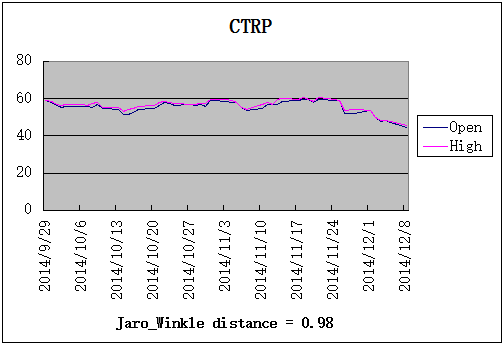
\includegraphics[width=3in]{figures/CTRP}
\caption{Stock time series snapshot for CTRP}
\vspace{1mm}
\end{figure}
\par

\par
\vspace{2mm}
 \begin{figure}[!h]
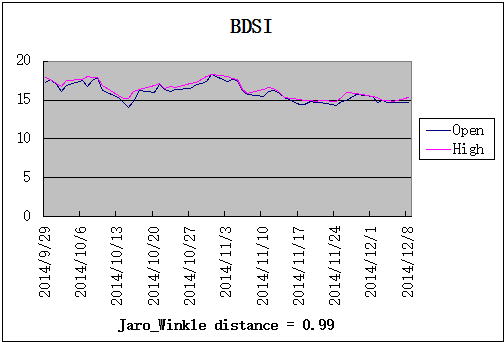
\includegraphics[width=3in]{figures/BDSI}
\caption{Stock time series snapshot for BDSI}
\vspace{1mm}
\end{figure}
\par

\vspace{1mm}
\par
Next, we set a $k=$ 7 time window, which means that we are going to evaluation similarity between two stocks in a longer period. First we keep the 50 date training dataset and get stock CZNC, OCLR and STRM as JSM's most similar stocks, shown in Figure 5, 6 and 7.
\par
 \begin{figure}[!h]
\vspace{2mm}
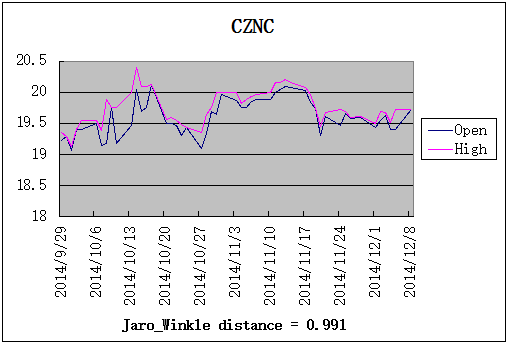
\includegraphics[width=3in]{figures/CZNC}
\caption{Stock time series snapshot for CZNC}
\vspace{1mm}
\end{figure}
\par

\par
 \begin{figure}[!h]
\vspace{2mm}
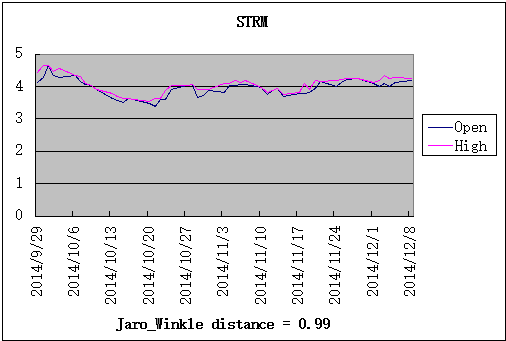
\includegraphics[width=3in]{figures/STRM}
\caption{Stock time series snapshot for STRM}
\vspace{1mm}
\end{figure}
\par

\par
 \begin{figure}[!h]
\vspace{2mm}
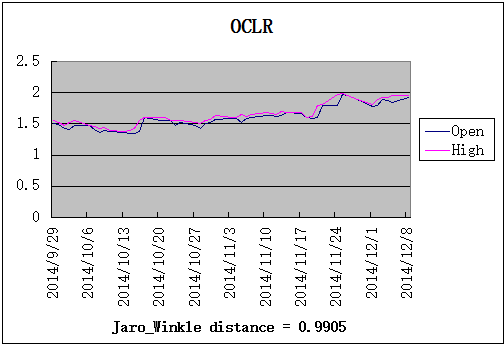
\includegraphics[width=3in]{figures/OCLR}
\caption{Stock time series snapshot for OCLR}
\vspace{1mm}
\end{figure}
\par

\vspace{1mm}
\par
As we can see from the figure,STRM still shows high similarity if we look at the general behavior of these two stocks, whereas CZNC and JSM shows a far apart behavior. After analyzing our algorithm, we found that for a long time window, we will need data from a longer time series for the string to be built. So we extend the training data space that the system is able to do a recommendation based on stock behavior in the last 1000 days. In that case, we are able to get the 3 most similar stocks:SPAR, CIFC and PLAB.\\
\par
 \begin{figure}[!h]
\vspace{2mm}
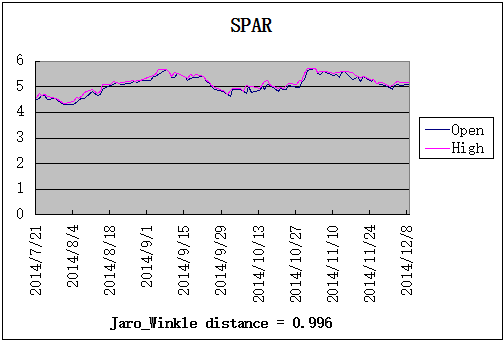
\includegraphics[width=3in]{figures/SPAR}
\caption{Stock time series snapshot for SPAR}
\vspace{1mm}
\end{figure}
\par

\par
 \begin{figure}[!h]
\vspace{2mm}
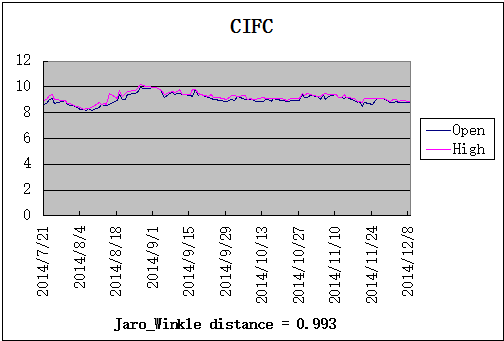
\includegraphics[width=3in]{figures/CIFC}
\caption{Stock time series snapshot for CIFC}
\vspace{1mm}
 \end{figure}
\par

\par
\vspace{2mm}
 \begin{figure}[!h]
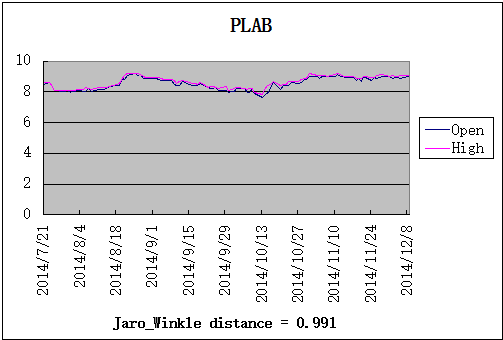
\includegraphics[width=3in]{figures/PLAB}
\caption{Stock time series snapshot for PLAB}
\vspace{1mm}
\end{figure}
\par

\vspace{1mm}
\par
An interesting finding about the result we get is that the general behavior of these three stocks seems similar to each other, but not quite the same as JSM. However, after looking at the graph with our criterion, we noticed that in each period of 7 days, the high price do follows the move of open price for both JSM and any of the recommended stocks, which means that we have already picked the similar stocks that matches the criterion best. However, a problem with this criterion is that it doesn't cover the behavior of JSM. Supposing that a user-selected stock doesn't show a long term behavior often, it is hard to find its similar stock correctly using such criterion.In that case, if we want recommendation to be correct enough, it is important for the user to choose a criterion that works well with the selected stock.\\ 


\section{Conclusion}
%Drew a conclusion of your project, describe the contributions of each team member in percentage and discuss future works.
Our stock recommendation system proposed a general framework for multiple events to predict two stocks\rq\  dependency. It allowed users to quickly find out their objective stocks from the screening results by three categories(market category, test issue, financial status) and check the most similar ones with their own favorite stocks. The time series of a stock is encoded as a string and stock similarity is measured based on string distances by Jaro Winkler Algorithm. The experiment results clearly reveal that the recommended stocks by our system indeed bear a similar trend with a certain given stock, thus prove the validity of our algorithm. \\

Future works of our project involves enable users to define different criterion to be described mathematically as set of events with restrictions on value and time. The contributions of each team member is: Yuechen Qin(25\%), Guangyang Zhang(25\%),Bowen Dang(25\%),Zheng Fang(25\%).


% An example of a floating figure using the graphicx package.
% Note that \label must occur AFTER (or within) \caption.
% For figures, \caption should occur after the \includegraphics.
% Note that IEEEtran v1.7 and later has special internal code that
% is designed to preserve the operation of \label within \caption
% even when the captionsoff option is in effect. However, because
% of issues like this, it may be the safest practice to put all your
% \label just after \caption rather than within \caption{}.
%
% Reminder: the "draftcls" or "draftclsnofoot", not "draft", class
% option should be used if it is desired that the figures are to be
% displayed while in draft mode.
%
%\begin{figure}[!t]
%\centering
%\includegraphics[width=2.5in]{myfigure}
% where an .eps filename suffix will be assumed under latex, 
% and a .pdf suffix will be assumed for pdflatex; or what has been declared
% via \DeclareGraphicsExtensions.
%\caption{Simulation Results}
%\label{fig_sim}
%\end{figure}

% Note that IEEE typically puts floats only at the top, even when this
% results in a large percentage of a column being occupied by floats.


% An example of a double column floating figure using two subfigures.
% (The subfig.sty package must be loaded for this to work.)
% The subfigure \label commands are set within each subfloat command, the
% \label for the overall figure must come after \caption.
% \hfil must be used as a separator to get equal spacing.
% The subfigure.sty package works much the same way, except \subfigure is
% used instead of \subfloat.
%
%\begin{figure*}[!t]
%\centerline{\subfloat[Case I]\includegraphics[width=2.5in]{subfigcase1}%
%\label{fig_first_case}}
%\hfil
%\subfloat[Case II]{\includegraphics[width=2.5in]{subfigcase2}%
%\label{fig_second_case}}}
%\caption{Simulation results}
%\label{fig_sim}
%\end{figure*}
%
% Note that often IEEE papers with subfigures do not employ subfigure
% captions (using the optional argument to \subfloat), but instead will
% reference/describe all of them (a), (b), etc., within the main caption.


% An example of a floating table. Note that, for IEEE style tables, the 
% \caption command should come BEFORE the table. Table text will default to
% \footnotesize as IEEE normally uses this smaller font for tables.
% The \label must come after \caption as always.
%
%\begin{table}[!t]
%% increase table row spacing, adjust to taste
%\renewcommand{\arraystretch}{1.3}
% if using array.sty, it might be a good idea to tweak the value of
% \extrarowheight as needed to properly center the text within the cells
%\caption{An Example of a Table}
%\label{table_example}
%\centering
%% Some packages, such as MDW tools, offer better commands for making tables
%% than the plain LaTeX2e tabular which is used here.
%\begin{tabular}{|c||c|}
%\hline
%One & Two\\
%\hline
%Three & Four\\
%\hline
%\end{tabular}
%\end{table}


% Note that IEEE does not put floats in the very first column - or typically
% anywhere on the first page for that matter. Also, in-text middle ("here")
% positioning is not used. Most IEEE journals/conferences use top floats
% exclusively. Note that, LaTeX2e, unlike IEEE journals/conferences, places
% footnotes above bottom floats. This can be corrected via the \fnbelowfloat
% command of the stfloats package.




% conference papers do not normally have an appendix


% use section* for acknowledgement
\section*{Acknowledgment}



Our group would like to thank Prof. Lin for providing us such an opportunity to explore the amazing world of big data. We\rq ve really learned a lot during this semester and this kind of experience is quite unforgettable and rewarding. Besides, we really appreciate the efforts of all the TAs. We\rq d like to thank them for their patience and great help during the semester.

\newpage
\appendix
\section{\\Title of Appendix A} \label{App:AppendixA}

Instructions on how to implement the application\\

\begin{enumerate}[label=\Alph*]

%step one
\item Project Composition\\

The project document has three folders: J2EE resources, jars and figures.\\

\begin{itemize}
\item The folder called J2EE resources contains all the elements we need inside the J2EE framework. Figure  9 shows how we organise these elements inside J2EE. It contains java packages, web contents and all the related structures.
\item The folder called jar contains all the jars needed to be installed into the lib of the WEB-INF folder inside J2EE framework.
\item The folder called figures contains the figure of the outcome of our UI.\\
\end{itemize}





%step two
\item Configuration steps:\\

 \begin{figure}[!h]
            \centering
           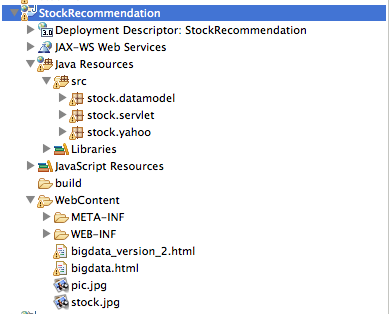
\includegraphics[width=0.5\textwidth]{figures/j2ee.jpg}
           \caption{info and like buttons}
          \vspace{0.1cm}
    \end{figure}
    
The folder called J2EE resources contains all the elements we need inside the J2EE framework. Figure  9 shows how we organise these elements inside J2EE. The step is as follows:\\
\begin{itemize}
\item Three java code packages are put inside "Java resources/src" folder. 
\item $bigdata\_version\_2.html$ and $stock.jpg$ are put inside WebContent/WEB-INF folder. 
\item jars are put inside the lib under WEB-INF folder.
\item Tomcat 7 is used as the server to run the project.\\
\end{itemize}

%step three
\item How to run the project:\\

 \begin{figure}[!h]
            \centering
           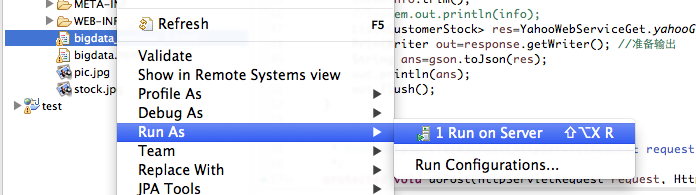
\includegraphics[width=0.5\textwidth]{figures/server.jpg}
           \caption{info and like buttons}
          \vspace{0.1cm}
    \end{figure}
    
\begin{itemize}
\item The project runs from $bigdata\_version\_2.html$. right click mouse, choose run as server and click finish, the UI webpage will appear in the browser at localhost:8080.
\item Client can make selections through the three drop-down buttons, which are market category, test issue and finical status.
\item After selection, by clicking the search button, the database will return all the stocks that fit in the prerequisites.
\item If client likes the stock, he can click the like button to add the symbol of the stock to the recommendation search bar.
\item Click recommend button will activate the system to calculate the similarities of all the stocks compared with clients\rq\ choice and presents the recommendation results in a table.
\item  The search bar on the top-right corner of the webpage is used to search for a specific stock.  If you type AAPL in the search bar, it will show you the stock information of apple.
\end{itemize}


\end{enumerate}






% trigger a \newpage just before the given reference
% number - used to balance the columns on the last page
% adjust value as needed - may need to be readjusted if
% the document is modified later
%\IEEEtriggeratref{8}
% The "triggered" command can be changed if desired:
%\IEEEtriggercmd{\enlargethispage{-5in}}

% references section

% can use a bibliography generated by BibTeX as a .bbl file
% BibTeX documentation can be easily obtained at:
% http://www.ctan.org/tex-archive/biblio/bibtex/contrib/doc/
% The IEEEtran BibTeX style support page is at:
% http://www.michaelshell.org/tex/ieeetran/bibtex/
%\bibliographystyle{IEEEtran}
% argument is your BibTeX string definitions and bibliography database(s)
%\bibliography{IEEEabrv,../bib/paper}
%
% <OR> manually copy in the resultant .bbl file
% set second argument of \begin to the number of references
% (used to reserve space for the reference number labels box)
%\begin{thebibliography}{a}

%\bibitem{IEEEhowto:kopka}
%H.~Kopka and P.~W. Daly, \emph{A Guide to \LaTeX}, 3rd~ed.\hskip 1em plus
 % 0.5em minus 0.4em\relax Harlow, England: Addison-Wesley, 1999.

%\end{thebibliography}
\renewcommand\refname{Reference}
\bibliographystyle{plain}
\bibliography{bare_conf}




% that's all folks
\end{document}


